\subsubsection{Inspiração biológica}

    O cérebro humano possui um tipo específico de célula que aparentemente nao se regenera lentamente como as outras. A estas células são atribuidas nossa capacidade de pensamento, lembranças e transferência de todo tipo de informações para todo o corpo. Estas células chamadas neurônios estão presentes em cifras de 100 bilhões de unidades. \cite{anderson1992artificial}
    O neurônio é dividido em basicamente três partes: núcleo, axônio e dendritos, e cada uma delas tem sua atividade bem estipulada. O núcleo é onde ocorre todo o processamento dos sinais elétricos recebidos pelos dendritos que ficam nas extremidades da célula e são transmitidos pelo axônio para o próximo neurônio.

    \begin{figure}[h]
        \centering
        \label{fig01}
            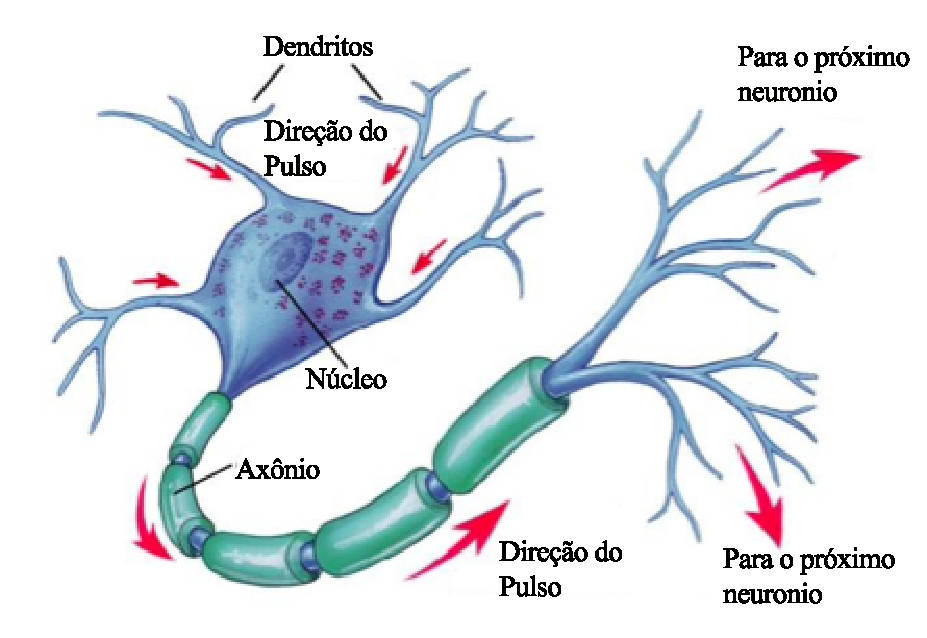
\includegraphics[keepaspectratio=true, scale=0.4]{editaveis/images/neuronio.eps}
        \caption{Representação de neurônio humano}
        Fonte: \url{http://goo.gl/vbd7T6}
    \end{figure}

    Estes pulsos, ou sinais elétricos, são transmitidos do axônio de um neurônio para os dendritos de um outro neurônio através das fendas sinapticas, ou sinápses.

    \begin{figure}[h]
        \centering
        \label{fig02}
            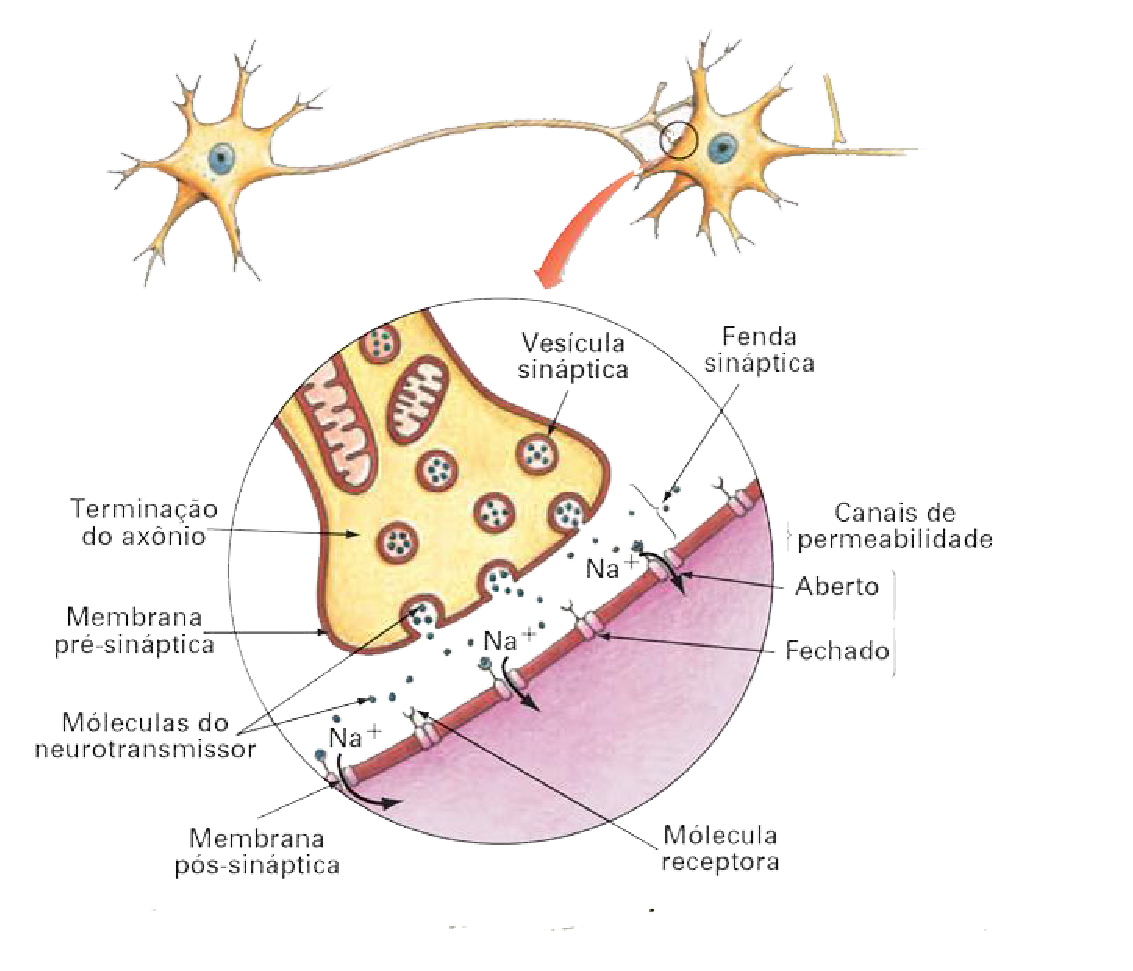
\includegraphics[keepaspectratio=true, scale=0.4]{editaveis/images/sinapse.eps}
        \caption{Representação de uma sinápse.}
        Fonte : \url{http://goo.gl/TCtvVG}
    \end{figure}

    As sinápses são regiões ativas eletroquimicamente entre as membranas celulares dos neurônios, onde a partir de uma excitação ocorre uma reação química que transmite os sinais de uma célula a outra por intermédio de substancias chamadas neurotransmissores.

\subsubsection{Modelagem matemática}
    O neurônio biológico pode ser modelado matematicamente de um modo que inspire a criação de um neurônio artificial a partir dessa divisão. Sendo assim, uma modelagem matemática de um neurônio biológico é: \cite{rocha2006}

    \begin{itemize}
        \item Entrada: São os dendritos, por onde os sinais chegam;
        \item Pesos: São as áreas onde as informações são transferidas de um neurônio para outro,  ou seja as sinápses;
        \item Soma: É o núcleo do neurônio, onde cada entrada é multiplicada com seu devido peso para que em seguida passe por uma função de transferência, a qual vai gerar os sinais de saída dos axônios;
        \item Função de Transferência: É o potencial necessário para ativação das fendas sinápticas.
        \item Saída: São os axônios do neurônio biológico.
    \end{itemize}

    Dessa maneira, tomando por base este modelo, o desenho de um neurônio artificial seria:

    \begin{figure}[h]
        \centering
        \label{fig03}
            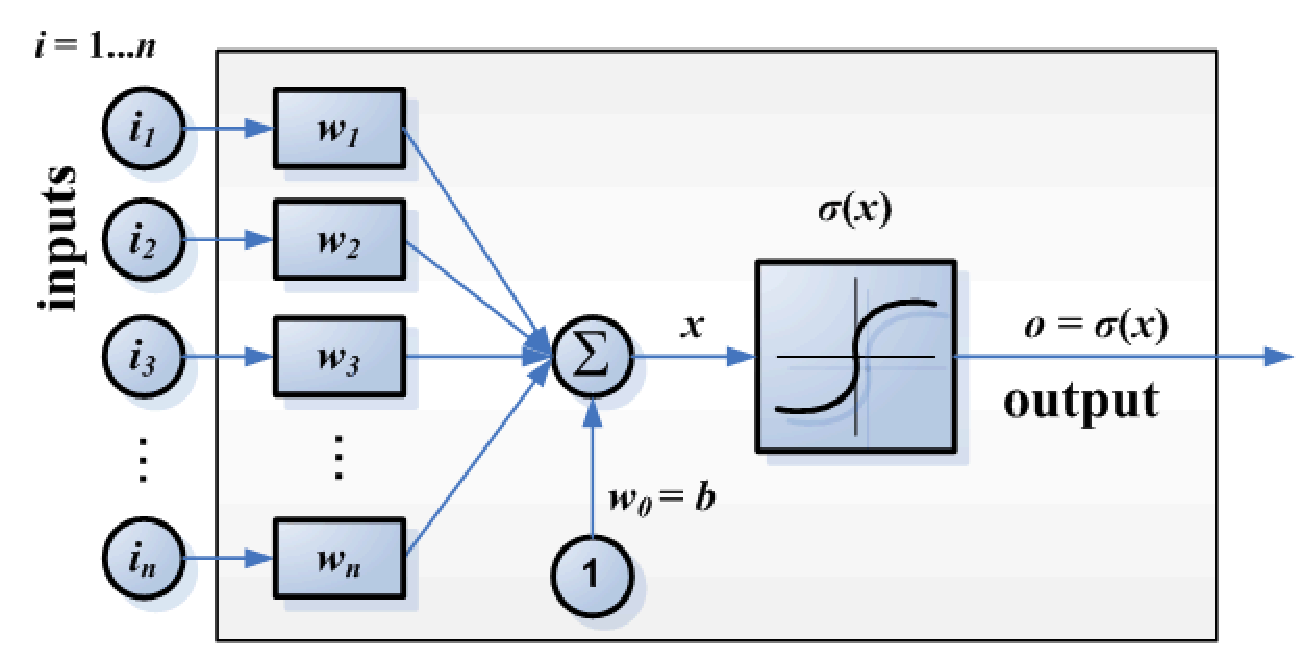
\includegraphics[keepaspectratio=true, scale=0.4]{editaveis/images/modeloNeuronio.eps}
        \caption{Representação matemática do neurônio.}
        Fonte : \url{http://goo.gl/iD2fg4}
    \end{figure}

\subsubsection{Perceptron de Multiplas Camadas}
    O \textit{perceptron} é a menor unidade de processamento, e representa um neurônio conforme a representação da figura 3(\ref{fig03}). Uma rede perceptron de multiplas camadas, ou MLP, é composta de camadas de perceptrons alinhados em diferentes camadas, que podem variar a partir de três. A primeira é a camada de entrada, por onde os dados entram na rede, a segunda é uma camada intermediária de processamento, normalmente chamada de camada escondida e a ultima é a camada dos neurônios de saída, que mostram a resposta. Um modelo básico de MLP é descrito na figura 4(\ref{fig04}) a seguir:

    \begin{figure}[h]
        \centering
        \label{fig04}
            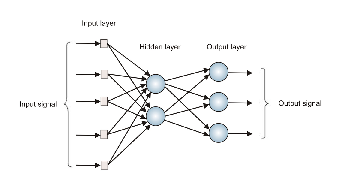
\includegraphics[keepaspectratio=true, scale=0.4]{editaveis/images/mlp.eps}
        \caption{Representação de uma MLP.}
        Fonte : \url{http://goo.gl/ICaZBQ}
    \end{figure}


